\chapter{Searching for the best existing solution}
Three parts composition brings in way more possibilities than two parts composition. 
But more possibilities also mean an increased computation complexity. The search space has been extended a lot by adding a whole new set of variables, and the time taken for a solution to be found might to be too elevated if one does not think about optimizing the search. In addition to that, adding a third voice to a composition is not bringing many new constraints (which would help discarding some potential solutions faster), but instead comes with many preferences, which in constraint programming, are translated to costs.

In addition, we need to find a way of arranging the costs in a way that comes as close as possible to what Fux was trying to express in his book. There are several ways to do this, which we will go through and discuss.  

This chapter will begin by explaining the search algorithm that is used to find a solution, continue by discussing the different ways of considering costs, and end by analysing the results that these different perspectives produce.

\section{Using Branch-And-Bound as a search algorithm}

To cope with the increased complexity brought about by the three-part composition, it was decided to switch from the Depth First Search algorithm (used in T. Wafflard's thesis) to a more efficient Branch and Bound (BAB). This allows us to handle costs properly and to find faster solutions. Moreover, the BAB algorithm can also produce non-optimal results, which is very valuable since finding the best overall solution can be time-consuming. When starting the search for a solution, it is now possible to ask for the next solution (i.e. a better solution than the one found previously, and if none was found previously, then just any valid solution), or for the best solution. In the latter case, the solver will continue to search until it finds the best solution or until it is stopped, returning a better solution each time it finds one.


\subsection{Heuristics}
When it comes to finding a solution, we obviously need some heuristics to guide the search, as there are so many different possibilities for a three-part composition. 
To know which heuristics we apply, we simply think about the most important variable to fix first. The most important 


\section{Designing the costs to be as faithful as possible to \gap} \label{costs}

Knowing that we are looking for the solution whose cost must be as low as possible, the question arises: how can we calculate the cost in order to best reflect the preferences expressed in \gap?

The way to translate each preference into a corresponding cost has of course been formalised in the previous sections, but that's not the crux of the matter. The question we face here is: what is the best way to combine all these individual costs to get the most accurate result in terms of what Fux is trying to convey?

Three main ways of doing this have been identified: a linear combination between costs, a search that minimises costs by lexicographic order, and a cost ordering that involves the calculation of minima. We will first describe each of these techniques and their respective advantages, and then compare them (and the results they produce).



\subsection{Linear Combination}


The first method of calculating our costs is a linear combination. This is the technique used in T. Wafflard's thesis. More precisely, it uses a linear combination in which all the weights are equal to one.



To be more precise about the method used to calculate the total cost in T. Wafflard's thesis, here is a more detailed explanation: there exists a total cost, $\tau$, which is equal to the sum of all individual costs, $\mathcal{C}$. The next step is to minimise $\tau$. Each $\mathcal{C}_i$ is usually itself a sum of sub-costs. Take, for example, the cost of motions, $\mathcal{C}_{motions} = \sum_j P_{costs}[j] $. This cost is the sum of all sub-costs of the motions (one per motion): by default, a contrary motion has a sub-cost of 0, an oblique motion has a sub-cost of 1 and a direct motion has a sub-cost of 2. These default values can be changed by the user to be set somewhere on a scale that ranges from $0$ to $64m$. For example, the user could set the oblique motion cost to be equal to $0$, and the cost for direct and contrary motion to be equal to $64m$, in order to get a composition filled with as many oblique motions as possible (always in accordance with the basic rules from \gap, i.e. all voices are never going to go in the same direction, see \ref{rule:same-movement}).

As mentioned at the beginning of this subsection, this procedure can be understood as a linear combination with weights of one only. However, since the cost factors are given different values according to the user's choices, this method is actually more like a regular linear combination, except that the weights are not multiplied by the costs once the latter have been set, but the costs are themselves made larger or smaller before the linear combination is calculated.

The linear combination has two major advantages: ease of implementation and high comprehensibility.


However, it has a major drawback: since the total cost $\tau$ we are minimising in a linear combination is the sum of all costs $\mathcal{C}$, the best solution might be a solution where one cost is absolutely huge and all the others are small. This might not be a problem if the outstanding cost is not really relevant, but if it is the cost of not using a harmonic triad, it goes completely against the preferences that Fux conveys in his work, making the solution inappropriate. A representation of this situation can be found in the figure \ref{fig:outstanding-cost}.

\begin{figure}[h]
    \centering
    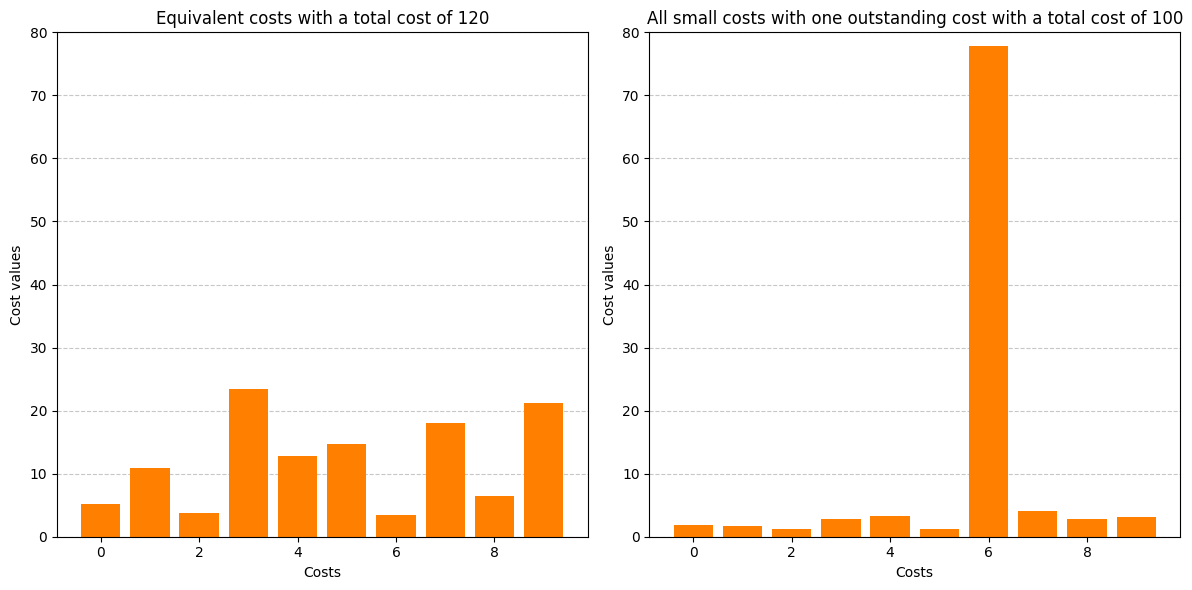
\includegraphics[width=1\textwidth]{Images/outstanding-costs.png}
    \caption{Example of a situation where a solution with an outstanding cost is preferred to a solution with equivalent low costs when using a linear combination}
    \label{fig:outstanding-cost}
\end{figure}

Another drawback of linear combination is that the result is pretty and unpredictable: changing the value of the cost may or may not make a difference, and you may need to set huge values to see a real effect. For example, if a composer really wants oblique motion, they may be forced to set the cost of the other types of motion to a huge value, or they may not see the difference between the default solution and their personalised solution. This is due to the fact that all the costs are mixed together and form an indistinguishable soup that the solver considers as a whole, and a small increase in the cost of the direct and contrary motions is very likely to be absorbed into this soup without any change being noticed.

These two drawbacks make the linear combination solution for the costs hardly acceptable when it comes to representing the preferences.
We will therefore examine the other two options for adjusting costs.

\subsection {Minimising the maxima}
In order to overcome the problem of outstanding costs that we encountered when considering the linear combination solution, one might consider using some minimums when calculating $\tau$, the total cost. For example, $\tau$ could be the maximum of all costs. By doing this, the solver would try to find a solution where the focus is on the worst cost and try to reduce it before trying to reduce the other costs.

The problem with this method arises when one cost is significantly higher than the others because it has been defined that way. Let's go back to our example of the composer wanting as many oblique motions as possible. You will set the cost for direct motion and contrary motion to the highest possible cost and start the search. As we've already discussed, it is not possible to have only oblique motions, since this would contradict the rule that not all voices can move in the same direction (\ref{rule:same-movement}). As a result, there will always be contrary motions, and since the cost for them has been set very high, it would be impossible for the solver to converge to a good solution. This creates a bottleneck effect, where once the solver has reached the best potential value of the worst cost, it cannot continue to find better solutions. 

\begin{figure}[h]
    \centering
    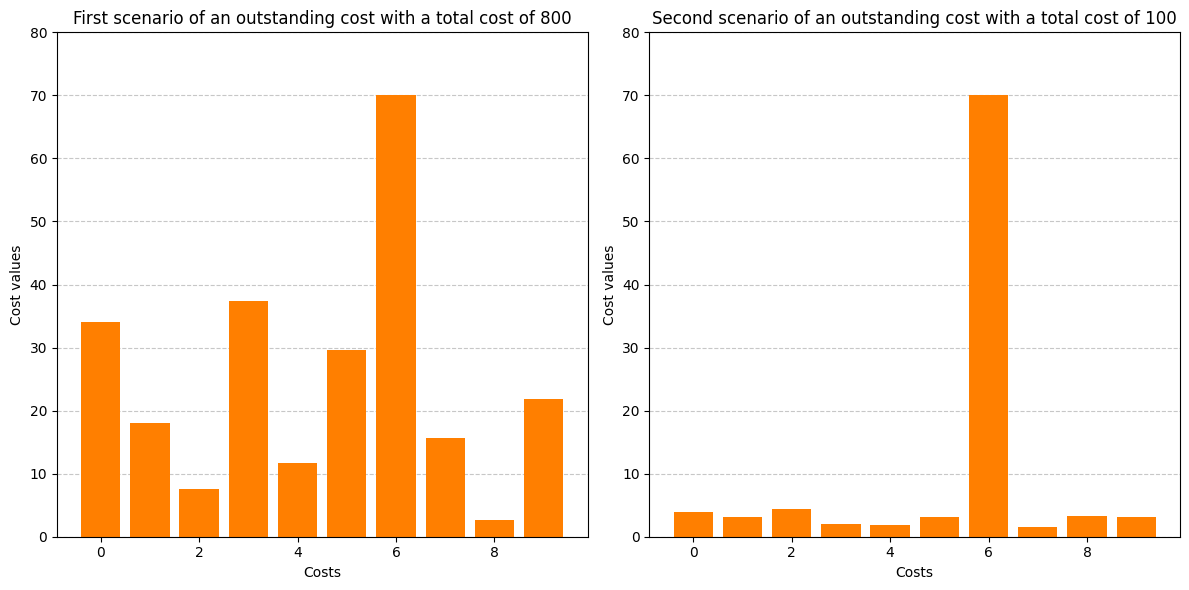
\includegraphics[width=1\textwidth]{Images/minimising-maxima.png}
    \caption{Example of two situations where one costs causes a bottleneck in the search as the solver cannot differn a situation where a solution with an outstanding cost is preferred to a solution with equivalent low costs when using a linear combination}
    \label{fig:outstanding-cost}
\end{figure}


Furthermore, even when considering a less extreme case (e.g. the default setting), this method requires a normalisation of the costs: there are $3\times (m-2)$ sub-costs for the variety cost, $3\times (m-1)$ sub-costs for the motion cost, but only $m$ sub-costs for the octave cost. This means that without normalisation, the motion cost will be on average three times larger than the octave cost, which means that the solver will put three times more effort into minimising the motion cost than the octave cost, which is unfair and unpractical.


\subsection{Lexicographical Order}\label{section:lexicographical-order}
The second way of dealing with the costs is to arrange them in an array and then perform a lexicographic minimisation. In other words, the costs would be arranged in order of importance: from most important to least important. The most important cost to minimise would be placed first in this array, and the solver would only try to minimise the other costs if the first cost remained the same or decreased. This method makes a lot of sense when you think about the rules that emanate of \gap. For example, Fux says that perfect consonance can be achieved by direct motion if there is no other possibility. This means that, all other things being equal, we would prefer to achieve perfect consonance by oblique or contrary motion, but that between a bad solution (respecting almost no preferences) in which perfect consonance is not achieved by direct motion, and a good solution (respecting almost all preferences) in which perfect consonance is achieved by direct motion, we would choose the good solution. 

Some costs are also more important than others in absolute terms. For example, when Fux says that an imperfect consonance is preferred to a fifth, which is preferred to an octave. This amounts to lexicographically ranking the cost of using an octave first (because we really don't want octaves), and then the cost of using a fifth (and there is no cost of using an imperfect consonance, since Fux indicates that this is preferable).
\begin{figure}[h]
    \begin{equation}
        \begin{aligned}
            \tau = [\underset{\text{minimise this first}}{\underbrace{\mathcal{C}_\text{octaves}}}, \mathcal{C}_\text{fifths}]
        \end{aligned}
    \end{equation}
    \caption{Array of costs demonstrating the practicality of a lexicographical order solving.}
\end{figure}

A second example, which ties in particularly well with the first, is that Fux tells us that the harmonic triad must be used in every measure unless a rule forbids it. In saying this, he places the preference for the harmonic triad above all other preferences, because the only reason that can prevent the use of a harmonic triad is a fixed constraint (and not a preference). You'll notice that the harmonic triad consists of a fifth (which is a perfect consonant), so Fux is telling us that we'd rather use a fifth in a harmonic triad than an imperfect consonant outside a harmonic triad. The lexicographic order search is the only one that allows this kind of concept to be taken into account, because in a linear combination these two preferences would be mutually "exclusive"\footnote{In the sense that their effects would work against each other.}: the first preference would add a cost where the second preference would not, and the second preference would add a cost where the first would not.

\begin{figure}[h]
    \begin{equation}
        \begin{aligned}
            \tau = [& \underset{\text{\fontsize{7}{11}\selectfont{minimize this first}}}{\underbrace{\mathcal{C}_\text{harmonic\_triad}}}, \underset{\text{\fontsize{7}{11}\selectfont\parbox{4cm}{and start minimizing this only if it is not possible anymore to minimize the harmonic triad cost}}}{\underbrace{\mathcal{C}_\text{octaves}}},\quad  \mathcal{C}_\text{fifths}]
        \end{aligned}
    \end{equation}
    \caption{Array of costs demonstrating the practicality of a lexicographical order solving.}
\end{figure}

And in this way we can keep integrating the different costs until we get a full array $\tau$ with all the costs ordered in a lexicographical way.

Of course, it is not always as simple as in the examples above, because it is not always easy to determine which cost has priority over which other. Sometimes Fux is very clear about it (e.g. for the harmonic triad cost, which Fux says has priority over everything else), and sometimes he isn't (do we prefer no off-key notes, or as much variety as possible?) This is a disadvantage of this method, because we have to hierarchise the costs, even if the choice is difficult. What's more, once the costs are ranked, their order becomes absolute and the solver loses some of its flexibility.

Knowing this, we made a suggested order that should be as close as possible to Fux's preferred order (or at least what we understood him to convey as his preferred order in \gap). This order should of course be changeable at the composer's discretion. The default order we have agreed upon is as follows:

\begin{multicols}{2}
    \begin{enumerate}
        \item $\mathcal{C}_\text{no\_syncope}$\footnote{The cost of not using a syncope in the fourth species.}
        \item $\mathcal{C}_\text{harmonic\_triad}$
        \item $\mathcal{C}_\text{harmonic\_triad\_3rd\_species}$
        \item $\mathcal{C}_\text{octaves}$
        \item $\mathcal{C}_\text{penult\_thesis\_is\_fifth}$\footnote{A specific cost for the second species, which applies when a penultimate thesis note does not make a fifth interval with the lowest stratum.}
        \item $\mathcal{C}_\text{fifths}$
        \item $\mathcal{C}_\text{off\_key}$\footnote{The cost of using sharps or flats.}
        \item $\mathcal{C}_\text{variety}$
        \item $\mathcal{C}_\text{m2\_eq\_zero}$\footnote{The cost of having the same note in the downbeat and the upbeat.}
        \item $\mathcal{C}_\text{not\_cambiata}$\footnote{The cost of not using a \textit{cambiata} if it is possible. The \textit{cambiata} can be characterised by the following scheme: \texttt{consonance - dissonance - consonance}.}
        \item $\mathcal{C}_\text{motions}$
        \item $\mathcal{C}_\text{m\_degrees}$\footnote{The cost of using big or small melodic intervals.}        
        \item $\mathcal{C}_\text{direct\_move\_to\_p\_cons}$
    \end{enumerate}
\end{multicols}

Some notes on the proposed order: 
\begin{itemize}
    \item One cost comes even before the harmonic triad cost, namely: the $\mathcal{C}_\text{no\_syncope}$ cost. This cost is at the heart of the fourth species, and a fourth species counterpoint without syncopations is not really a fourth species counterpoint. This is why syncope is considered even more important than the harmonic triad.
    \item The cost of $\mathcal{C}_\text{penult\_thesis\_is\_fifth}$ comes before the cost of $\mathcal{C}_\text{fifths}$, as it is an exception to the latter (similar to the interaction explained above in the section between $\mathcal{C}_\text{harmonic\_triad}$ and $\mathcal{C}_\text{fifths})$.
    
    \item $\mathcal{C}_\text{off\_key}$ was added to its ranking because it is actually an absolute rule not to use off-key notes, but Fux does use some, and so it was decided to put this cost after the very important costs to allow off-key notes to happen.

    \item The costs $\mathcal{C}_\text{variety}$, $\mathcal{C}_\text{motions}$ and $\mathcal{C}_\text{m\_degrees}$ were ranked in order from least to most restrictive. First we say that we would prefer the note to change as much as possible (with the variety cost), then we indicate our preference for the direction (with the motion cost), and finally we indicate our preference for the size of the motion (with the melodic interval cost). This gives the solver as much flexibility as possible. The other way round would have been more restrictive, since the solver would have minimised the melodic intervals first, setting them all to one, which doesn't leave much room for the motion cost to have an effect, and forcing the variety cost to be high in any case, as with  intervals the melody tends to vary only a little.
    
    \item $\mathcal{C}_\text{m2\_eq\_zero}$ and $\mathcal{C}_\text{m\_degrees}$ were classified right after the variety cost as they are an in-measure variation of the variety preference.

\end{itemize}


\paragraph{NB} Please note that using the lexicographic order does not \textit{not} mean that the last costs are not taken into account, they will be \textit{too} minimised by the solver. It just means that if the solver has to choose between minimising one cost or another, it will minimise the first one in the lexicographic order. 

\subsection{Comparison between the three types of costs.}

We have now discussed the advantages and disadvantages of each of the three methods. These are all listed in \ref{tab:comparison}. As you can see, no one method is definitively better than another, and the only way to know which method is better in practice is to \textit{test} them in practice to find out which of the methods gives the best results. 

\begin{center}
    \centering
    \captionof{table}{Comparison of Three Methods According to Criteria}
    \label{tab:comparison}
    \begin{tabularx}{\textwidth}{|>{\centering\arraybackslash}p{4cm}|>{\centering\arraybackslash}X|>{\centering\arraybackslash}X|>{\centering\arraybackslash}X|}
        \hline
        \textbf{Criteria} & \textbf{Linear Combination} & \textbf{Minimising the maximum} & \textbf{Lexicographic Search} \\
        \hline
        Outsanding costs & \cellcolor{red!25}Yes & \cellcolor{green!25}No & \cellcolor{orange!25}Only for minor costs \\
        \hline
        Predictability\footnote{Changing a cost has a big impact on the result.} & \cellcolor{red!25}No & \cellcolor{orange!25}Some & \cellcolor{green!25}Yes \\
        \hline
        One cost might be a bottleneck & \cellcolor{green!25}No & \cellcolor{red!25}Yes & \cellcolor{green!25}No \\
        \hline
        Need to normalise costs& \cellcolor{green!25}No & \cellcolor{red!25}Yes & \cellcolor{green!25}No \\
        \hline
        Possibility to ensure a preference of one cost over another  & \cellcolor{red!25}No & \cellcolor{red!25}No & \cellcolor{green!25}Yes \\
        \hline
        Need for hierarchisation of costs & \cellcolor{green!25}No & \cellcolor{green!25}No & \cellcolor{red!25}Yes \\
        \hline
        Flexibility & \cellcolor{orange!25}Medium & \cellcolor{green!25}High & \cellcolor{red!25}Low \\
        \hline

    \end{tabularx}
\end{center}

Even more, one could think about a combination of all the methods to get rid of their disadvantages. In fact, we could enjoy the advantages of all the methods by combining them and cleverly designing a lexicographical order search in which the cost is a linear combination of a maximum minimisation.

\subsection{Experimenting with the three types}
To experiment which method gives the best results, we will follow this plan: start with a purely lexicographical order, using the default preference order as defined in \ref{section:lexicographical-order}, then solve the problem of which preference is more important than the other by grouping them in the same cell of the lexicographical order (either by linear combination or by maximum minimisation).


These experiments are carried out using two different counterbalancing combination setups. The first setup is a combination of two first-species counterpoints, since this is the basic case of three-part composition. The second setup is a combination of a third species counterpoint and a fourth species counterpoint. This setup was chosen because it's rich enough to capture the complexity of counterpoint writing, but not too rich, like the fifth species, which makes the way it works more opaque and difficult to analyse.

